\documentclass[a4paper,12pt]{article}
\usepackage[T1]{fontenc}
\usepackage[utf8]{inputenc}
\usepackage{lmodern}
\usepackage[spanish]{babel}
\usepackage{textcomp}
\usepackage{amsmath}
\usepackage{amsfonts}
\usepackage[framed,numbered,autolinebreaks]{mcode}
\usepackage{amssymb}
\usepackage{graphicx}
\usepackage{caption}
\usepackage{subcaption}
\usepackage{float}
\usepackage{color}
\usepackage{mcode}
\usepackage[left=2cm,right=2cm,top=2cm,bottom=2cm]{geometry}
\usepackage{fancyhdr}
\title{Modelado de un rectificador de onda usando la serie de Fourier}
\author{
  Aguilar Enriquez Paul Sebastian\\
  Cabrera López Oscar Emilio
}

\pagestyle{fancy}
\fancyhf{}
\lhead[]{}
\chead[]{}
\rfoot{\thepage}
\lfoot[]{}
\cfoot[]{}

\linespread{1.3}

\renewcommand\headrule
{{\color[RGB]{98,36,35}%
    \hrule height 2pt
    width\headwidth
    \vspace{1.3pt}%
    \hrule height 1pt
    width\headwidth
  }}
  \addto\captionsspanish{\def\tablename{Tabla}}%imprime Tabla en lugar de Cuadro
  %%
  \spanishdecimal{.}


\begin{document}
\thispagestyle{fancy}
\maketitle
\newpage
\tableofcontents
\newpage

\section{Introducción}

\subsection{Jean-Baptiste Joseph Fourier}
\indent Jean-Baptiste Joseph Fourier (21 March 1768 – 16 May 1830) fue un físico y matemático francés, entre sus aportaciones a la ciencia están la series de Fourier para representar cualquier función periódica mediante una serie de senos y cosenos, y ampliamente usada para resolver problemas sobre vibraciones y la transferencia de calor; la transformada de Fourier y la ley de Fourier.\\
\indent En diciembre de 1807, Joseph Fourier presentó ante la Academia de Ciencias de París su \textit{Théorie de la propagation de la chaleur dans le solides}, en ella proponía una ecuación diferencial para describir la difusión del calor en un cuerpo sólido y propuso una solución mediante la representación de una función como series de senos y cosenos.\\
\indent Este trabajo fue ampliamente criticado en su momento, especialmente por Biot, Poisson, Laplace y Lagrange, quién se oponía a la idea de que una función cualquiera pudiese ser representada mediante una serie trigonométrica.\\
\indent Fourier veía a las matemáticas como una herramienta para explicar el mundo, y con su análisis pretendía únicamente plantear un fenómeno físico y explicar su solución, y no llegar a un rigor matemático en su desarrollo.

\subsection{El rectificador de onda completa}
\indent Tanto la generación como la transmisión y conversión de energía eléctrica se realizan de una manera más simple y eficiente en corriente alterna. Asimismo, debido a la resistencia de los conductores que forman una línea de transmisión, es conveniente que la corriente sea lo menor posible, lo cual requiere aumentar la tensión. Los transformadores de corriente alterna permiten llevar a cabo esta conversión con alto rendimiento.\\
\indent Sin embargo, la gran mayoría de los aparatos eléctricos y electrónicos precisan de un flujo de tensión continua, este flujo es suministrado por un sistema llamado fuente de alimentación. El componente más importante de una fuente de alimentación es el rectificador de onda, cuya función es convertir la corriente alterna en una corriente unidireccional, que idealmente, no variará con el tiempo.\\
\indent Existen dos tipos principales de rectificadores, el rectificador de media onda y el de onda completa. El circuito rectificador de media onda tiene como ventaja su sencillez, pero no permite utilizar toda la energía disponible, ya que los
semiciclos negativos son desaprovechados. Este inconveniente se resuelven con los rectificadores de onda completa.\\
\indent Como se ha señalado anteriormente, los rectificadores ideales producen formas de onda unidireccionales pero de ninguna manera constantes, como sería deseable para su uso como fuente de alimentación. Dado que el problema es equivalente al de eliminar las componentes frecuenciales diferentes de la continua, la solución consiste en utilizar un filtro pasabajos cuya frecuencia de corte esté suficientemente por debajo de la
frecuencia de la onda rectificada, dicho filtro puede implementarse mediante capacitores o inductores, aquí analizaremos el segundo caso.

\section{Objetivos}
\begin{enumerate}
    \item Mostrar una aplicación de la serie trigonométrica de Fourier, relacionada con las carreras de la DIE.
    \item Dar una ligera introducción a la respuesta de sistemas en frecuencia.
    \item Comprender el funcionamiento de un rectificador de onda.
    \item Analizar el comportamiento de un circuito RL aplicado a un rectificador de corriente.
    \item Calcular los coeficientes de la serie de Fourier de una señal eléctrica.
    \item Aplicar los conocimientos adquiridos en clase sobre la serie de Fourier para señales periódicas pares e impares.
    \item Obtener la serie de Fourier de una señal rectificada.
    \item Interpretar el significado de la serie y los coeficientes de la serie de Fourier.
    \item Valorar la contribución de Fourier al análisis de fenómenos fisicos.    
\end{enumerate}

\section{Desarrollo}

La idea básica de las series de Fourier es que toda función periódica de período $T$ puede ser expresada como una suma trigonométrica de senos y cosenos del mismo período $T$.\\
\indent A mediados del siglo XVIII, es decir, unos cincuenta años antes de los trabajos de Fourier, ya se había planteado el problema de la representación de una función por medio de una serie trigonométrica.\\
\indent En 1747 mientras estudiaba el movimiento en las cuerdas de violín d´Alembert muestra que la solución general de la ecuación de ondas
\[ \frac{\partial ^2u}{\partial t^2}-\alpha\frac{\partial^2u}{\partial x^2} = 0 \]
se escribe de la forma
\[ u(x,t) = \varphi(x + \alpha t) + \psi(x - \alpha t)  \]
A continuación impone la condición de que los extremos de la cuerda en $x = 0$ y $x = l$ estén fijos y deduce que
\[ u(x, t) = \varphi(\alpha t + x) - \varphi(\alpha t - x) \quad y \quad \varphi(x) = \varphi(2l + x). \]
Esa solución fue también demostrada por Euler en 1749. Euler difería con D’Alembert en el tipo de funciones iniciales que podían tenerse en cuenta. De hecho, estas diferencias pueden considerarse como una de las primeras
manifestaciones escritas sobre los problemas que ha llevado consigo la definición de función, continuidad, dominio de definición, etc. La influencia de la teoría de las series trigonométricas en la clarificación de estos conceptos fue determinante.\\
\indent Taylor había observado ya en 1715 que las funciones $sen\left( \frac{n\pi x}{l}\right), cos\left(\frac{n\pi \alpha t}{l}\right)$ con $n$ entero son soluciones de la ecuación y se anulan en $x = 0$ y $x = l$, lo que explica que una cuerda, además de su tono fundamental, puede dar también el tono fundamental de las cuerdas de longitud $1/2$, $1/3$, $1/4$,. . . de la original. Esto llevó a Bernoulli a considerar que la cuerda podía vibrar según la expresión
\[ u(x,t) = \sum _n a_n sen\left( \frac{n\pi x}{l}\right)cos\left(\frac{n\pi \alpha t}{l}\right)(t-\beta_n)\]
y como todas las modificaciones observadas del fenómeno se podían explicar partiendo de esta ecuación, consideró que daba la solución general.\\
\indent El trabajo siguiente al de Bernoulli en las Memorias de la Academia de Ciencias de Berlín era de Euler, quien aseguraba frente a d´Alembert que la función $\varphi$ puede ser completamente arbitraria entre $-l$ y $l$ y señalaba que la solución de Bernoulli era general si y sólo si cualquier curva arbitraria entre $0$ y $l$ podía ser representada por una serie trigonométrica.\\
\indent La fórmula
\[ a_n = \int_0^1 \varphi(x)sen\left(n\pi x\right)dx \]
para calcular los coeficientes $a_n$ apareció por primera vez en un artículo escrito por Euler en 1777.
\indent Lagrange, joven aún, entró en escena en 1759. Estudió las vibraciones de un hilo sin masa al que se coloca una cantidad finita de masas de igual magnitud equidistribuidas y vio cómo variaban las vibraciones al tender el
número de masas a infinito; tras largas manipulaciones analíticas decidió que la solución de Euler era correcta.\\
\indent La contribución de Fourier comenzó en 1807 con sus estudios del problema
del flujo del calor
\[ \frac{\partial u}{\partial t} = \frac{1}{2}\frac{\partial^2u}{\partial x^2} \]
presentado a la Académie des Sciences en 1811 y publicado en parte como la célebre \textit{Théorie analytique de la chaleur} en 1822. Fourier hizo un intento serio por demostrar que cualquier función diferenciable puede ser expandida
en una serie trigonométrica.

\subsection{Rectificador}
\indent Dada la necesidad de convertir la corriente alterna en continua, lo cual se logra por medio de la rectificación.\\
\indent Un rectificador es el elemento o circuito que permite convertir la corriente alterna en corriente continua. Esto se realiza ya sea utilizando diodos rectificadores, semiconductores de estado sólido, válvulas al vacío o válvulas gaseosas como las de vapor de mercurio, asi como con circuitos RC o LC que funcionan como circuitos filtradores de señales.\\
\indent Dependiendo de las características de la alimentación en corriente alterna que emplean, se les clasifica en monofásicos, cuando están alimentados por una fase de la red eléctrica, o trifásicos cuando se alimentan por tres fases.\\
\indent Atendiendo al tipo de rectificación, pueden ser de media onda, cuando sólo se utiliza uno de los semiciclos de la corriente, o de onda completa, donde ambos semiciclos son aprovechados.\\

\indent Existen una gran variedad de rectificadores, entre los mas comunes se encuentran los siguientes:
\begin{enumerate}
    \item Rectificador de Media Onda
    \item Rectificador de Onda Completa con Tap Central
    \item Rectificador de Onda Completa con Puente de Diodos
    \item Rectificador de Onda (Media o Completa) con filtros RC o LC
\end{enumerate}

\subsubsection{Rectificador de onda completa}
\indent Un rectificador de onda completa es un circuito empleado para convertir una señal de corriente alterna de entrada (Vi) en corriente continua de salida (Vo) pulsante. En este caso, la parte negativa de la señal se convierte en positiva o bien la parte positiva de la señal se convertirá en negativa, según se necesite una señal positiva o negativa de corriente continua.\\

\textbf{Rectificador con Tap Central (Dos diodos)}

\indent En el circuito de la figura, ambos diodos no pueden encontrarse simultáneamente en directa o en inversa, ya que las diferencias de potencial a las que están sometidos son de signo contrario; por tanto uno se encontrará polarizado inversamente y el otro directamente. La tensión de entrada (Vi) es, en este caso, la media de la tensión del secundario del transformador. Figura \ref{Figura1}\\

\textbf{Tensión de entrada positiva} \indent El diodo 1 se encuentra en polarización directa(conduce), mientras que el 2 se encuentra en inversa (no conduce). La tensión de salida es igual a la de entrada.Nota:los diodos en posición directa conducen altas corrientes,en posición inversa alta tensiones. Figura \ref{Figura2}\\

\textbf{Tensión de entrada negativa} \indent El diodo 2 se encuentra en polarización directa (conduce), mientras que el diodo 1 se encuentra en polarización inversa (no conduce). La tensión de salida es igual a la de entrada pero de signo contrario. El diodo 1 ha de soportar en inversa la tensión máxima del secundario. Figura \ref{Figura3}\\

\begin{figure}
  \begin{center}
    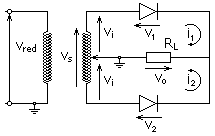
\includegraphics{images/Circuito_rectificador_onda_completa.png}
    \caption{Circuito rectificador de onda completa}
    \label{Figura1}
  \end{center}
\end{figure}

\begin{figure}
  \begin{center}
    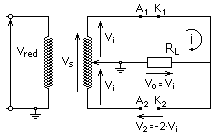
\includegraphics{images/Circuito_rectificador_onda_completa_ON.png}
    \caption{Circuito rectificador de onda completa ON}
    \label{Figura2}
  \end{center}
\end{figure}

\begin{figure}
  \begin{center}
    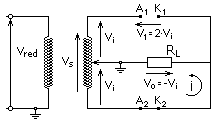
\includegraphics{images/Circuito_rectificador_onda_completa_OFF.png}
    \caption{Circuito rectificador de onda completa OFF}
    \label{Figura3}
  \end{center}
\end{figure}

\begin{figure}
  \begin{center}
    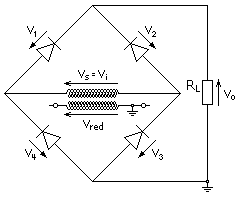
\includegraphics{images/Puente_de_diodos.png}
    \caption{Circuito rectificador de onda completa con puente de diodos}
    \label{Figura4}
  \end{center}
\end{figure}

.\\

\textbf{Rectificador con Puente de Graetz (Puente de diodos)}

\indent En este caso se emplean cuatro diodos con la disposición de la figura \ref{Figura4}. Al igual que antes, sólo son posibles dos estados de conducción, o bien los diodos 1 y 3 están en directa y conducen (tensión positiva) o por el contrario son los diodos 2 y 4 los que se encuentran en directa y conducen (tensión negativa).\\

\indent A diferencia del caso anterior, ahora la tensión máxima de salida es la del secundario del transformador (el doble de la del caso anterior), la misma que han de soportar los diodos en inversa, al igual que en el rectificador con dos diodos. Esta es la configuración usualmente empleada para la obtención de onda continua.\\

\subsubsection{Rectificador de onda completa de filtro inductivo}

\indent Los rectificadores ideales (que utilizan diodos, como los mostrados anteriormente) producen formas de onda unidireccionales pero de ninguna manera constantes, como sería deseable para su uso como fuente de alimentación. Dado que el problema es equivalente al de eliminar las componentes frecuenciales diferentes de la continua, la solución consiste en utilizar un filtro pasabajos cuya frecuencia de corte esté suficientemente por debajo de la
frecuencia de la onda rectificada.\\

\begin{figure}
  \begin{center}
    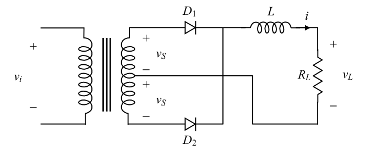
\includegraphics{images/Circuito_Inductivo_Onda_Completa.png}
    \caption{Circuito rectificador inductivo de onda completa}
    \label{Figura5}
  \end{center}
\end{figure}

\indent En la figura \ref{Figura5} podemos observar el circuito de la versión inductiva del rectificador de onda
completa.\\

\indent En este circuito la corriente por el inductor no se interrumpe nunca. En efecto, la tensión en el inductor seguiría la misma evolución de la tensión de entrada, internándose en la región negativa. Esto es posible porque por la naturaleza reactiva del inductor, puede tener tensión negativa y corriente positiva. Si ahora permitimos la aparición del segundo semiciclo rectificado, el diodo D2 se encontrará con una tensión que tiende a ser positiva en su ánodo (la de entrada rectificada) y negativa en su cátodo (la del inductor), por lo tanto estará en condiciones de conducir, inyectando en el inductor una corriente apropiada para mantener las condiciones de continuidad. En ese
momento, el diodo D 1 dejará de conducir, pues su polarización se volverá inversa, desvinculándose del inductor.\\

\indent En resumen, el inductor estará expuesto, ya sea por uno u otro diodo, a una fuente de tensión ideal correspondiente a una senoide rectificada. El análisis puede proceder ahora de acuerdo con la teoría de circuitos lineales, según el modelo indicado en la figura \ref{Figura6} .

\begin{figure}
  \begin{center}
    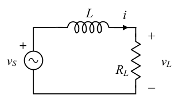
\includegraphics{images/Circuito_Inductivo_Lineal_Onda_Completa.png}
    \caption{Circuito rectificador inductivo de onda completa}
    \label{Figura6}
  \end{center}
\end{figure}

\section{Resultados}

\section{Conclusiones}

\section{Referencias}

\begin{thebibliography}{9}
\bibitem{Ref1}Federico Miyara. (2002). RECTIFICACIÓN. 23/05/2016, de Universidad Nacional de Rosario Sitio web: http://www.fceia.unr.edu.ar/enica3/rectif.pdf
\bibitem{Ref2}-. (-). Rectificador. 23/05/2016, de Wikipedia Sitio web: https://es.wikipedia.org/wiki/Rectificador
%\bibitem{Ref3}-. (-). Circuitos Rectificadores. 23/05/2016, de Universidad Nacional Abierta y a Distancia Sitio web: http://datateca.unad.edu.co/contenidos/243006/Contenidos/Circuitos_con_diodos/circuitos_rectificadores.html
%\bibitem{Ref4}-. (-). Rectificador de onda completa. 23/05/2016, de Wikipedia Sitio web: https://es.wikipedia.org/wiki/Rectificador_de_onda_completa
\end{thebibliography}

\end{document}
